\documentclass[12pt,a4paper]{article}
\usepackage{graphicx}
\usepackage{amsmath}
\usepackage{bm}
\usepackage{interval}
\usepackage{amssymb}
\usepackage{float}
\usepackage{subfigure}
\usepackage{titlesec}
\usepackage{tikz}
% \usepackage{algorithm}
\usepackage[linesnumbered,boxed]{algorithm2e}
% \usepackage{algorithmic}
\usepackage[noend]{algpseudocode}
\usepackage{epsfig}
\usepackage[letterpaper,top=2cm,bottom=2cm,left=3cm,right=3cm,marginparwidth=1.75cm]{geometry}
\usepackage[colorlinks=true, allcolors=blue]{hyperref}

% Inputs, Initialize settings
\algnewcommand{\Inputs}[1]{%
  \State \textbf{Inputs:}
  \Statex \hspace*{\algorithmicindent}\parbox[t]{.8\linewidth}{\raggedright #1}
}
\algnewcommand{\Initialize}[1]{%
  \State \textbf{Initialize:}
  \Statex \hspace*{\algorithmicindent}\parbox[t]{.8\linewidth}{\raggedright #1}
}

% Change section font size
\titleformat{\section}  % which section command to format
  {\fontsize{14}{16}\bfseries} % format for whole line
  {\thesection} % how to show number
  {1em} % space between number and text
  {} % formatting for just the text
  [] % formatting for after the text

\title{DS Written Homework 5}
\author{Student ID: b10201054}

\begin{document}
\maketitle

\section{Binary Heap Operation}

\begin{enumerate}
    \item [(a)] $\Rightarrow$ means inserting next node, $\rightarrow$ means swimming.
        \begin{figure}[!ht]
        \centering
        \begin{minipage}{0.07\textwidth}
            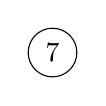
\begin{tikzpicture}
                % Nodes
                \node[circle, draw] (7) at (0,0) {7};
            \end{tikzpicture}
        \end{minipage}
        \begin{minipage}{0.03\textwidth}
            $\Rightarrow$
        \end{minipage}
        \begin{minipage}{0.14\textwidth}
            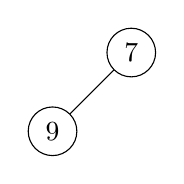
\begin{tikzpicture}
                % Nodes
                \node[circle, draw] (7) at (0,0) {7};
                \node[circle, draw] (9) at (-1,-1) {9};
                % Edges
                \draw[-] (7) -- (9);
            \end{tikzpicture}
        \end{minipage}
        \begin{minipage}{0.03\textwidth}
            $\Rightarrow$
        \end{minipage}
        \begin{minipage}{0.18\textwidth}
            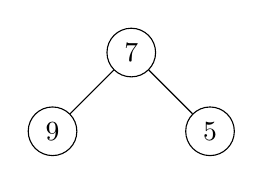
\begin{tikzpicture}
                % Nodes
                \node[circle, draw] (7) at (0,0) {7};
                \node[circle, draw] (9) at (-1,-1) {9};
                \node[circle, draw] (5) at (1,-1) {5};
                % Edges
                \draw[-] (7) -- (9);
                \draw[-] (7) -- (5);
            \end{tikzpicture}
        \end{minipage}
        \begin{minipage}{0.03\textwidth}
            $\rightarrow$
        \end{minipage}
        \begin{minipage}{0.18\textwidth}
            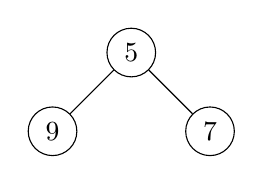
\begin{tikzpicture}
                % Nodes
                \node[circle, draw] (5) at (0,0) {5};
                \node[circle, draw] (9) at (-1,-1) {9};
                \node[circle, draw] (7) at (1,-1) {7};
                % Edges
                \draw[-] (5) -- (9);
                \draw[-] (5) -- (7);
            \end{tikzpicture}
        \end{minipage}
        \begin{minipage}{0.03\textwidth}
            $\Rightarrow$
        \end{minipage}
        
        \end{figure}
        \begin{figure}[!ht]
            \centering
            \begin{minipage}{0.21\textwidth}
                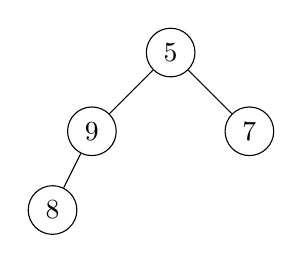
\begin{tikzpicture}
                    % Nodes
                    \node[circle, draw] (5) at (0,0) {5};
                    \node[circle, draw] (9) at (-1,-1) {9};
                    \node[circle, draw] (7) at (1,-1) {7};
                    \node[circle, draw] (8) at (-1.5,-2) {8};
                    % Edges
                    \draw[-] (5) -- (9);
                    \draw[-] (5) -- (7);
                    \draw[-] (9) -- (8);
                \end{tikzpicture}
            \end{minipage}
            \begin{minipage}{0.03\textwidth}
                $\rightarrow$
            \end{minipage}
            \begin{minipage}{0.21\textwidth}
                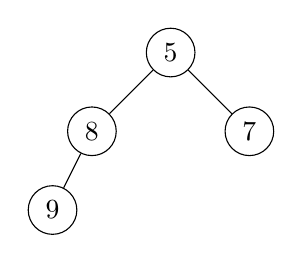
\begin{tikzpicture}
                    % Nodes
                    \node[circle, draw] (5) at (0,0) {5};
                    \node[circle, draw] (8) at (-1,-1) {8};
                    \node[circle, draw] (7) at (1,-1) {7};
                    \node[circle, draw] (9) at (-1.5,-2) {9};
                    % Edges
                    \draw[-] (5) -- (8);
                    \draw[-] (5) -- (7);
                    \draw[-] (8) -- (9);
                \end{tikzpicture}
            \end{minipage}
            \begin{minipage}{0.03\textwidth}
                $\Rightarrow$
            \end{minipage}
            \begin{minipage}{0.21\textwidth}
                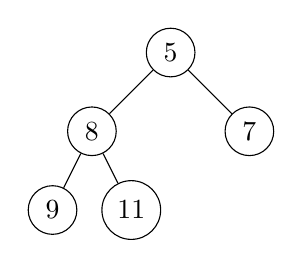
\begin{tikzpicture}
                    % Nodes
                    \node[circle, draw] (5) at (0,0) {5};
                    \node[circle, draw] (8) at (-1,-1) {8};
                    \node[circle, draw] (7) at (1,-1) {7};
                    \node[circle, draw] (9) at (-1.5,-2) {9};
                    \node[circle, draw] (11) at (-0.5,-2) {11};
                    % Edges
                    \draw[-] (5) -- (8);
                    \draw[-] (5) -- (7);
                    \draw[-] (8) -- (9);
                    \draw[-] (8) -- (11);
                \end{tikzpicture}
            \end{minipage}
            \begin{minipage}{0.03\textwidth}
                $\Rightarrow$
            \end{minipage}
            \begin{minipage}{0.21\textwidth}
                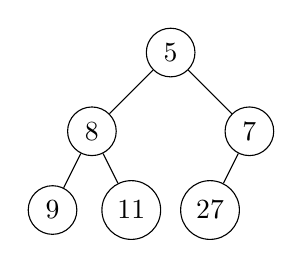
\begin{tikzpicture}
                    % Nodes
                    \node[circle, draw] (5) at (0,0) {5};
                    \node[circle, draw] (8) at (-1,-1) {8};
                    \node[circle, draw] (7) at (1,-1) {7};
                    \node[circle, draw] (9) at (-1.5,-2) {9};
                    \node[circle, draw] (11) at (-0.5,-2) {11};
                    \node[circle, draw] (27) at (0.5,-2) {27};
                    % Edges
                    \draw[-] (5) -- (8);
                    \draw[-] (5) -- (7);
                    \draw[-] (8) -- (9);
                    \draw[-] (8) -- (11);
                    \draw[-] (7) -- (27);
                \end{tikzpicture}
            \end{minipage}
        \end{figure}
        \begin{figure}[!ht]
            \centering
            \begin{minipage}{0.03\textwidth}
                $\Rightarrow$
            \end{minipage}
            \begin{minipage}{0.25\textwidth}
                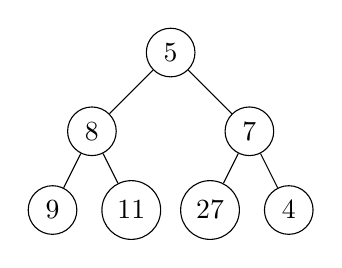
\begin{tikzpicture}
                    % Nodes
                    \node[circle, draw] (5) at (0,0) {5};
                    \node[circle, draw] (8) at (-1,-1) {8};
                    \node[circle, draw] (7) at (1,-1) {7};
                    \node[circle, draw] (9) at (-1.5,-2) {9};
                    \node[circle, draw] (11) at (-0.5,-2) {11};
                    \node[circle, draw] (27) at (0.5,-2) {27};
                    \node[circle, draw] (4) at (1.5,-2) {4};
                    % Edges
                    \draw[-] (5) -- (8);
                    \draw[-] (5) -- (7);
                    \draw[-] (8) -- (9);
                    \draw[-] (8) -- (11);
                    \draw[-] (7) -- (27);
                    \draw[-] (7) -- (4);
                \end{tikzpicture}
            \end{minipage}
            \begin{minipage}{0.03\textwidth}
                $\rightarrow$
            \end{minipage}
            \begin{minipage}{0.25\textwidth}
                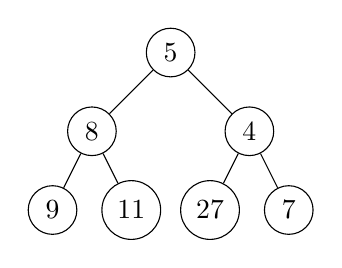
\begin{tikzpicture}
                    % Nodes
                    \node[circle, draw] (5) at (0,0) {5};
                    \node[circle, draw] (8) at (-1,-1) {8};
                    \node[circle, draw] (4) at (1,-1) {4};
                    \node[circle, draw] (9) at (-1.5,-2) {9};
                    \node[circle, draw] (11) at (-0.5,-2) {11};
                    \node[circle, draw] (27) at (0.5,-2) {27};
                    \node[circle, draw] (7) at (1.5,-2) {7};
                    % Edges
                    \draw[-] (5) -- (8);
                    \draw[-] (5) -- (4);
                    \draw[-] (8) -- (9);
                    \draw[-] (8) -- (11);
                    \draw[-] (4) -- (27);
                    \draw[-] (4) -- (7);
                \end{tikzpicture}
            \end{minipage}
            \begin{minipage}{0.03\textwidth}
                $\rightarrow$
            \end{minipage}
            \begin{minipage}{0.25\textwidth}
                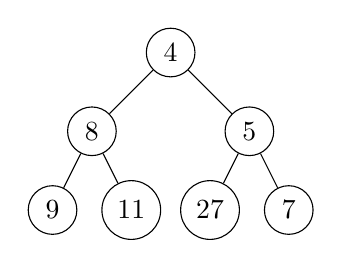
\begin{tikzpicture}
                    % Nodes
                    \node[circle, draw] (4) at (0,0) {4};
                    \node[circle, draw] (8) at (-1,-1) {8};
                    \node[circle, draw] (5) at (1,-1) {5};
                    \node[circle, draw] (9) at (-1.5,-2) {9};
                    \node[circle, draw] (11) at (-0.5,-2) {11};
                    \node[circle, draw] (27) at (0.5,-2) {27};
                    \node[circle, draw] (7) at (1.5,-2) {7};
                    % Edges
                    \draw[-] (4) -- (8);
                    \draw[-] (4) -- (5);
                    \draw[-] (8) -- (9);
                    \draw[-] (8) -- (11);
                    \draw[-] (5) -- (27);
                    \draw[-] (5) -- (7);
                \end{tikzpicture}
            \end{minipage}
            \begin{minipage}{0.03\textwidth}
                $\Rightarrow$
            \end{minipage}
        \end{figure}
        \begin{figure}[!ht]
            \centering
            \begin{minipage}{0.37\textwidth}
                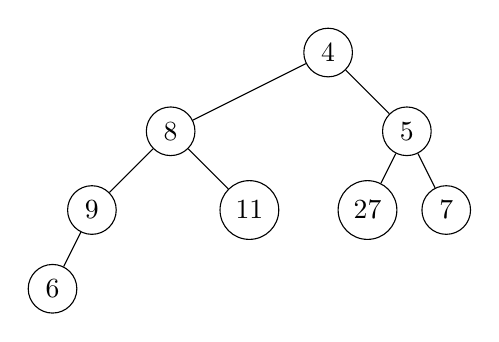
\begin{tikzpicture}
                    % Nodes
                    \node[circle, draw] (4) at (0,0) {4};
                    \node[circle, draw] (8) at (-2,-1) {8};
                    \node[circle, draw] (5) at (1,-1) {5};
                    \node[circle, draw] (9) at (-3,-2) {9};
                    \node[circle, draw] (11) at (-1,-2) {11};
                    \node[circle, draw] (27) at (0.5,-2) {27};
                    \node[circle, draw] (7) at (1.5,-2) {7};
                    \node[circle, draw] (6) at (-3.5,-3) {6};
                    % Edges
                    \draw[-] (4) -- (8);
                    \draw[-] (4) -- (5);
                    \draw[-] (8) -- (9);
                    \draw[-] (8) -- (11);
                    \draw[-] (5) -- (27);
                    \draw[-] (5) -- (7);
                    \draw[-] (9) -- (6);
                \end{tikzpicture}
            \end{minipage}
            \begin{minipage}{0.03\textwidth}
                $\rightarrow$
            \end{minipage}
            \begin{minipage}{0.37\textwidth}
                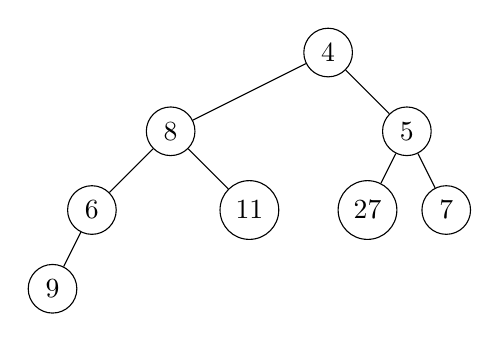
\begin{tikzpicture}
                    % Nodes
                    \node[circle, draw] (4) at (0,0) {4};
                    \node[circle, draw] (8) at (-2,-1) {8};
                    \node[circle, draw] (5) at (1,-1) {5};
                    \node[circle, draw] (6) at (-3,-2) {6};
                    \node[circle, draw] (11) at (-1,-2) {11};
                    \node[circle, draw] (27) at (0.5,-2) {27};
                    \node[circle, draw] (7) at (1.5,-2) {7};
                    \node[circle, draw] (9) at (-3.5,-3) {9};
                    % Edges
                    \draw[-] (4) -- (8);
                    \draw[-] (4) -- (5);
                    \draw[-] (8) -- (6);
                    \draw[-] (8) -- (11);
                    \draw[-] (5) -- (27);
                    \draw[-] (5) -- (7);
                    \draw[-] (6) -- (9);
                \end{tikzpicture}
            \end{minipage}
        \end{figure}
        \begin{figure}[!ht]
            \centering
            \begin{minipage}{0.03\textwidth}
                $\rightarrow$
            \end{minipage}
            \begin{minipage}{0.37\textwidth}
                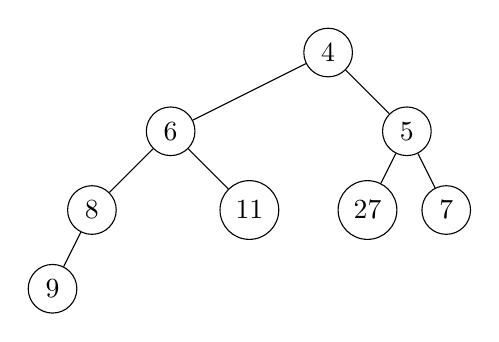
\begin{tikzpicture}
                    % Nodes
                    \node[circle, draw] (4) at (0,0) {4};
                    \node[circle, draw] (6) at (-2,-1) {6};
                    \node[circle, draw] (5) at (1,-1) {5};
                    \node[circle, draw] (8) at (-3,-2) {8};
                    \node[circle, draw] (11) at (-1,-2) {11};
                    \node[circle, draw] (27) at (0.5,-2) {27};
                    \node[circle, draw] (7) at (1.5,-2) {7};
                    \node[circle, draw] (9) at (-3.5,-3) {9};
                    % Edges
                    \draw[-] (4) -- (6);
                    \draw[-] (4) -- (5);
                    \draw[-] (6) -- (8);
                    \draw[-] (6) -- (11);
                    \draw[-] (5) -- (27);
                    \draw[-] (5) -- (7);
                    \draw[-] (8) -- (9);
                \end{tikzpicture}
            \end{minipage}
            \begin{minipage}{0.03\textwidth}
                $\Rightarrow$
            \end{minipage}
            \begin{minipage}{0.37\textwidth}
                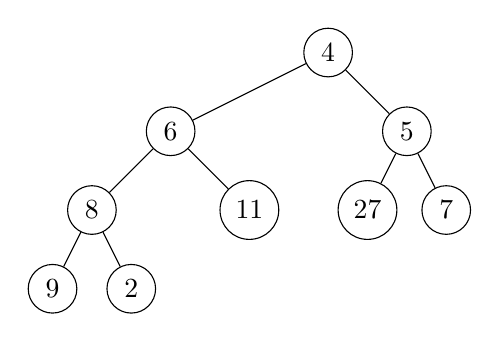
\begin{tikzpicture}
                    % Nodes
                    \node[circle, draw] (4) at (0,0) {4};
                    \node[circle, draw] (6) at (-2,-1) {6};
                    \node[circle, draw] (5) at (1,-1) {5};
                    \node[circle, draw] (8) at (-3,-2) {8};
                    \node[circle, draw] (11) at (-1,-2) {11};
                    \node[circle, draw] (27) at (0.5,-2) {27};
                    \node[circle, draw] (7) at (1.5,-2) {7};
                    \node[circle, draw] (9) at (-3.5,-3) {9};
                    \node[circle, draw] (2) at (-2.5,-3) {2};
                    % Edges
                    \draw[-] (4) -- (6);
                    \draw[-] (4) -- (5);
                    \draw[-] (6) -- (8);
                    \draw[-] (6) -- (11);
                    \draw[-] (5) -- (27);
                    \draw[-] (5) -- (7);
                    \draw[-] (8) -- (9);
                    \draw[-] (8) -- (2);
                \end{tikzpicture}
            \end{minipage}
        \end{figure}
        \begin{figure}[!ht]
            \centering
            \begin{minipage}{0.03\textwidth}
                $\rightarrow$
            \end{minipage}
            \begin{minipage}{0.37\textwidth}
                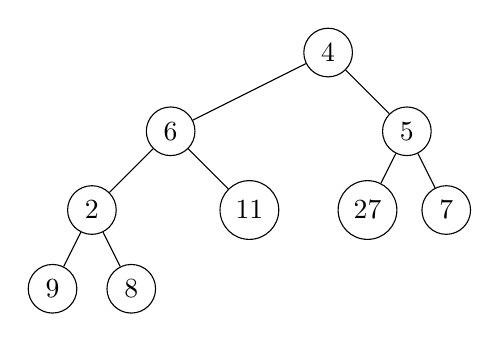
\begin{tikzpicture}
                    % Nodes
                    \node[circle, draw] (4) at (0,0) {4};
                    \node[circle, draw] (6) at (-2,-1) {6};
                    \node[circle, draw] (5) at (1,-1) {5};
                    \node[circle, draw] (2) at (-3,-2) {2};
                    \node[circle, draw] (11) at (-1,-2) {11};
                    \node[circle, draw] (27) at (0.5,-2) {27};
                    \node[circle, draw] (7) at (1.5,-2) {7};
                    \node[circle, draw] (9) at (-3.5,-3) {9};
                    \node[circle, draw] (8) at (-2.5,-3) {8};
                    % Edges
                    \draw[-] (4) -- (6);
                    \draw[-] (4) -- (5);
                    \draw[-] (6) -- (2);
                    \draw[-] (6) -- (11);
                    \draw[-] (5) -- (27);
                    \draw[-] (5) -- (7);
                    \draw[-] (2) -- (9);
                    \draw[-] (2) -- (8);
                \end{tikzpicture}
            \end{minipage}
            \begin{minipage}{0.03\textwidth}
                $\rightarrow$
            \end{minipage}
            \begin{minipage}{0.37\textwidth}
                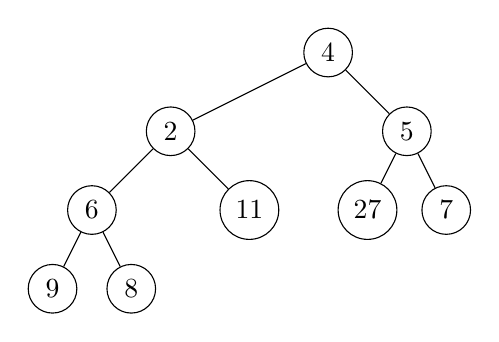
\begin{tikzpicture}
                    % Nodes
                    \node[circle, draw] (4) at (0,0) {4};
                    \node[circle, draw] (2) at (-2,-1) {2};
                    \node[circle, draw] (5) at (1,-1) {5};
                    \node[circle, draw] (6) at (-3,-2) {6};
                    \node[circle, draw] (11) at (-1,-2) {11};
                    \node[circle, draw] (27) at (0.5,-2) {27};
                    \node[circle, draw] (7) at (1.5,-2) {7};
                    \node[circle, draw] (9) at (-3.5,-3) {9};
                    \node[circle, draw] (8) at (-2.5,-3) {8};
                    % Edges
                    \draw[-] (4) -- (2);
                    \draw[-] (4) -- (5);
                    \draw[-] (2) -- (6);
                    \draw[-] (2) -- (11);
                    \draw[-] (5) -- (27);
                    \draw[-] (5) -- (7);
                    \draw[-] (6) -- (9);
                    \draw[-] (6) -- (8);
                \end{tikzpicture}
            \end{minipage}
        \end{figure}
        \begin{figure}[!ht]
            \centering
            \begin{minipage}{0.03\textwidth}
                $\rightarrow$
            \end{minipage}
            \begin{minipage}{0.37\textwidth}
                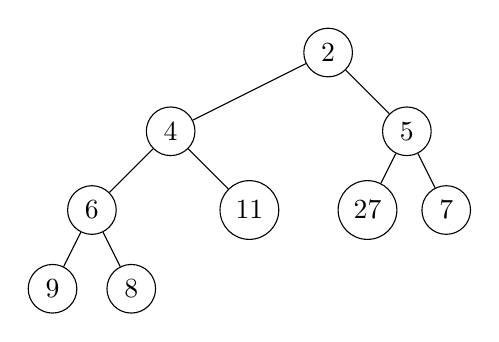
\begin{tikzpicture}
                    % Nodes
                    \node[circle, draw] (2) at (0,0) {2};
                    \node[circle, draw] (4) at (-2,-1) {4};
                    \node[circle, draw] (5) at (1,-1) {5};
                    \node[circle, draw] (6) at (-3,-2) {6};
                    \node[circle, draw] (11) at (-1,-2) {11};
                    \node[circle, draw] (27) at (0.5,-2) {27};
                    \node[circle, draw] (7) at (1.5,-2) {7};
                    \node[circle, draw] (9) at (-3.5,-3) {9};
                    \node[circle, draw] (8) at (-2.5,-3) {8};
                    % Edges
                    \draw[-] (2) -- (4);
                    \draw[-] (2) -- (5);
                    \draw[-] (4) -- (6);
                    \draw[-] (4) -- (11);
                    \draw[-] (5) -- (27);
                    \draw[-] (5) -- (7);
                    \draw[-] (6) -- (9);
                    \draw[-] (6) -- (8);
                \end{tikzpicture}
            \end{minipage}
        \end{figure}
        \newpage
    \item [(b)] $\Rightarrow$ means inserting next node, $\rightarrow$ means swimming.
        \begin{figure}[!ht]
            \centering
            \begin{minipage}{0.37\textwidth}
                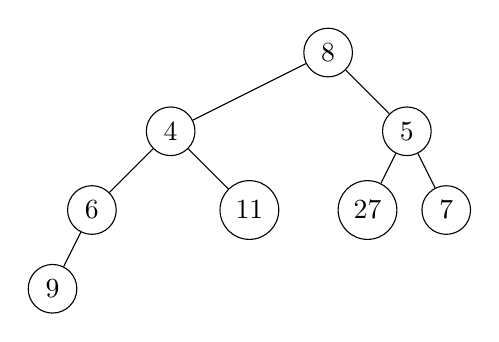
\begin{tikzpicture}
                    % Nodes
                    \node[circle, draw] (8) at (0,0) {8};
                    \node[circle, draw] (4) at (-2,-1) {4};
                    \node[circle, draw] (5) at (1,-1) {5};
                    \node[circle, draw] (6) at (-3,-2) {6};
                    \node[circle, draw] (11) at (-1,-2) {11};
                    \node[circle, draw] (27) at (0.5,-2) {27};
                    \node[circle, draw] (7) at (1.5,-2) {7};
                    \node[circle, draw] (9) at (-3.5,-3) {9};
                    % Edges
                    \draw[-] (8) -- (4);
                    \draw[-] (8) -- (5);
                    \draw[-] (4) -- (6);
                    \draw[-] (4) -- (11);
                    \draw[-] (5) -- (27);
                    \draw[-] (5) -- (7);
                    \draw[-] (6) -- (9);
                \end{tikzpicture}
            \end{minipage}
            \begin{minipage}{0.03\textwidth}
                $\rightarrow$
            \end{minipage}
            \begin{minipage}{0.37\textwidth}
                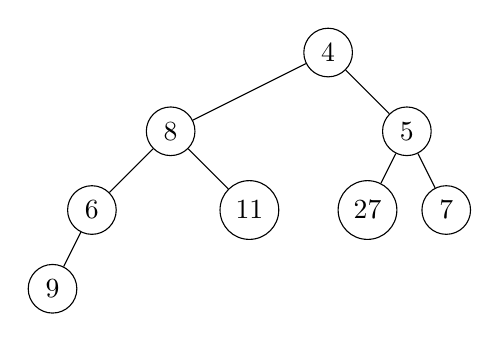
\begin{tikzpicture}
                    % Nodes
                    \node[circle, draw] (4) at (0,0) {4};
                    \node[circle, draw] (8) at (-2,-1) {8};
                    \node[circle, draw] (5) at (1,-1) {5};
                    \node[circle, draw] (6) at (-3,-2) {6};
                    \node[circle, draw] (11) at (-1,-2) {11};
                    \node[circle, draw] (27) at (0.5,-2) {27};
                    \node[circle, draw] (7) at (1.5,-2) {7};
                    \node[circle, draw] (9) at (-3.5,-3) {9};
                    % Edges
                    \draw[-] (4) -- (8);
                    \draw[-] (4) -- (5);
                    \draw[-] (8) -- (6);
                    \draw[-] (8) -- (11);
                    \draw[-] (5) -- (27);
                    \draw[-] (5) -- (7);
                    \draw[-] (6) -- (9);
                \end{tikzpicture}
            \end{minipage}
        \end{figure}
        \begin{figure}[!ht]
            \centering
            \begin{minipage}{0.03\textwidth}
                $\rightarrow$
            \end{minipage}
            \begin{minipage}{0.37\textwidth}
                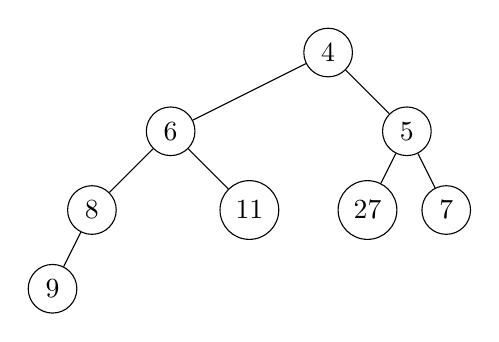
\begin{tikzpicture}
                    % Nodes
                    \node[circle, draw] (4) at (0,0) {4};
                    \node[circle, draw] (6) at (-2,-1) {6};
                    \node[circle, draw] (5) at (1,-1) {5};
                    \node[circle, draw] (8) at (-3,-2) {8};
                    \node[circle, draw] (11) at (-1,-2) {11};
                    \node[circle, draw] (27) at (0.5,-2) {27};
                    \node[circle, draw] (7) at (1.5,-2) {7};
                    \node[circle, draw] (9) at (-3.5,-3) {9};
                    % Edges
                    \draw[-] (4) -- (6);
                    \draw[-] (4) -- (5);
                    \draw[-] (6) -- (8);
                    \draw[-] (6) -- (11);
                    \draw[-] (5) -- (27);
                    \draw[-] (5) -- (7);
                    \draw[-] (8) -- (9);
                \end{tikzpicture}
            \end{minipage}
        \end{figure}
\end{enumerate}

\section{Binomial Heap}    

\begin{enumerate}
    \item [(a)] 
        If there are two same degree binomial trees, we will merge them into a degree + 1 binomial tree.
        If binomial heap contains 10 bionomial trees, their degree must be different, so if we want the smallest number of nodes, we can choose smallest 10 numbers of the degree.
        Hence, the smallest possible number of nodes is $\sum_{k=0}^{9} 2^k = 2^10 - 1 = 1023$.
    \item [(b)]
        Insert a node has $O(1)$ complexity.
        
        Merge two trees has $O(1)$ complexity.

        Insert m node has m insertion and at most $\log_{2}m$ merge.(Without considering the trees already in heap.)

        The worst case of inserting time complexity happens when we need to merge all the binomial trees in the current binomial heap.
        By (a) we can find the largest possible number of an n nodes binomial heap is $N = \log_{2}n$.

        Hence, the time complexity of inserting m node is $O(m + \log_{2}m + \log_{2}n) = O(m + \log n)$.
        
\end{enumerate}

\section{Fibonacci Heap}    

\begin{enumerate}
    \item [(a)] Result:
        \begin{enumerate}
            \item [Step 1.] Extract Min = 3:
                \begin{figure}[!ht]
                    \centering
                    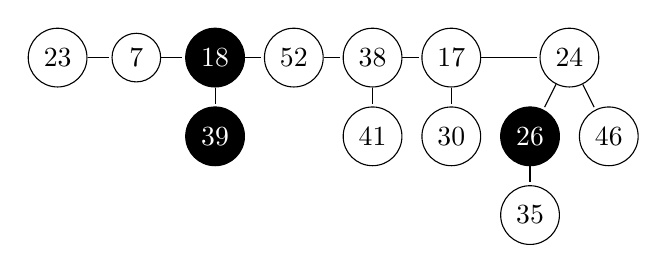
\begin{tikzpicture}[scale=0.5,shorten >=1pt]
                        % Nodes
                        \node[circle, draw] (23) at (-1,0) {23};
                        \node[circle, draw] (7) at (1,0) {7};
                        \node[circle, draw] (17) at (9,0) {17};
                        \node[circle, draw] (24) at (12,0) {24};
                        \node[circle, draw, fill=black, text=white] (18) at (3,0) {18};
                        \node[circle, draw, fill=black, text=white] (39) at (3,-2) {39};
                        \node[circle, draw] (52) at (5,0) {52};
                        \node[circle, draw] (38) at (7,0) {38};
                        \node[circle, draw] (41) at (7,-2) {41};
                        \node[circle, draw] (30) at (9, -2) {30};
                        \node[circle, draw, fill=black, text=white] (26) at (11,-2) {26};
                        \node[circle, draw] (35) at (11,-4) {35};
                        \node[circle, draw] (46) at (13,-2) {46};

                        % Edges
                        \draw[-] (23) -- (7);
                        \draw[-] (7) -- (18);
                        \draw[-] (18) -- (52);
                        \draw[-] (52) -- (38);
                        \draw[-] (38) -- (17);
                        \draw[-] (17) -- (24);
                        
                        \draw[-] (17) -- (30);
                        \draw[-] (24) -- (26);
                        \draw[-] (24) -- (46);

                        \draw[-] (18) -- (39);
                        \draw[-] (38) -- (41);
                        \draw[-] (26) -- (35);
                    \end{tikzpicture}
                \end{figure}
            \item [Step 2.] From the min = 17, record the root degree, find the same degree tree then merge them.
                In this case we record [(17, 1), (24, 2), (23, 0)], then the next node (7,0) is same degree as (23, 0), merge:
                \begin{figure}[!ht]
                    \centering
                    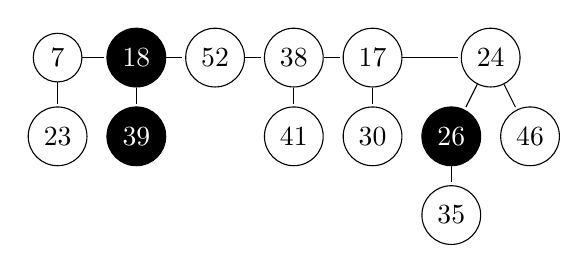
\begin{tikzpicture}[scale=0.5,shorten >=1pt]
                        % Nodes
                        \node[circle, draw] (7) at (1,0) {7};
                        \node[circle, draw] (23) at (1,-2) {23};
                        \node[circle, draw] (17) at (9,0) {17};
                        \node[circle, draw] (24) at (12,0) {24};
                        \node[circle, draw, fill=black, text=white] (18) at (3,0) {18};
                        \node[circle, draw, fill=black, text=white] (39) at (3,-2) {39};
                        \node[circle, draw] (52) at (5,0) {52};
                        \node[circle, draw] (38) at (7,0) {38};
                        \node[circle, draw] (41) at (7,-2) {41};
                        \node[circle, draw] (30) at (9, -2) {30};
                        \node[circle, draw, fill=black, text=white] (26) at (11,-2) {26};
                        \node[circle, draw] (35) at (11,-4) {35};
                        \node[circle, draw] (46) at (13,-2) {46};

                        % Edges
                        \draw[-] (7) -- (18);
                        \draw[-] (18) -- (52);
                        \draw[-] (52) -- (38);
                        \draw[-] (38) -- (17);
                        \draw[-] (17) -- (24);
                        
                        \draw[-] (7) -- (23);
                        \draw[-] (18) -- (39);
                        \draw[-] (38) -- (41);
                        \draw[-] (17) -- (30);
                        \draw[-] (24) -- (26);
                        \draw[-] (24) -- (46);

                        
                        \draw[-] (26) -- (35);
                    \end{tikzpicture}
                \end{figure}
            \newpage
            \item [Step 3.] 
                After merged, the list we recorded is [(17, 1), (24, 2)], find (7, 1) is same degree as (17, 1), merge:
                \begin{figure}[!ht]
                    \centering
                    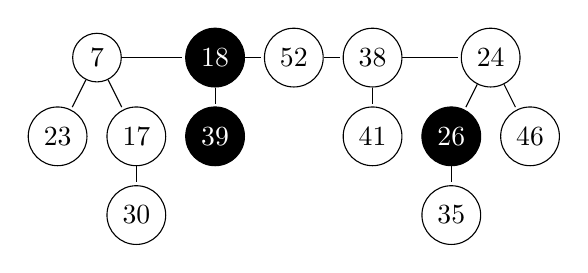
\begin{tikzpicture}[scale=0.5,shorten >=1pt]
                        % Nodes
                        \node[circle, draw] (7) at (1,0) {7};
                        \node[circle, draw] (23) at (0,-2) {23};
                        \node[circle, draw] (17) at (2,-2) {17};
                        \node[circle, draw] (30) at (2,-4) {30};
                        \node[circle, draw] (24) at (11,0) {24};
                        \node[circle, draw, fill=black, text=white] (18) at (4,0) {18};
                        \node[circle, draw, fill=black, text=white] (39) at (4,-2) {39};
                        \node[circle, draw] (52) at (6,0) {52};
                        \node[circle, draw] (38) at (8,0) {38};
                        \node[circle, draw] (41) at (8,-2) {41};
                        \node[circle, draw, fill=black, text=white] (26) at (10,-2) {26};
                        \node[circle, draw] (35) at (10,-4) {35};
                        \node[circle, draw] (46) at (12,-2) {46};

                        % Edges
                        \draw[-] (7) -- (18);
                        \draw[-] (18) -- (52);
                        \draw[-] (52) -- (38);
                        \draw[-] (38) -- (24);
                        
                        \draw[-] (7) -- (23);
                        \draw[-] (7) -- (17);
                        \draw[-] (18) -- (39);
                        \draw[-] (38) -- (41);
                        \draw[-] (17) -- (30);
                        \draw[-] (24) -- (26);
                        \draw[-] (24) -- (46);

                        
                        \draw[-] (26) -- (35);
                    \end{tikzpicture}
                \end{figure}
            \item [Step 4.] 
                After merged, the list we recorded is [(24, 2)], find (7, 2) is same degree as (24, 2), merge:
                \begin{figure}[!ht]
                    \centering
                    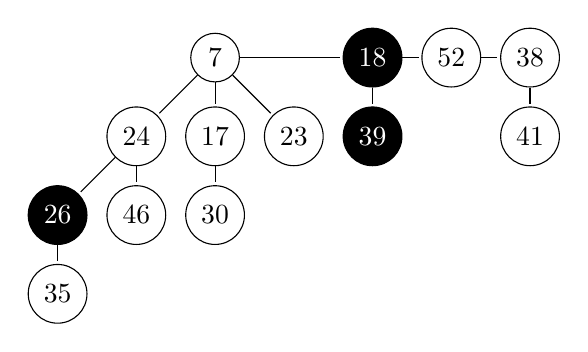
\begin{tikzpicture}[scale=0.5,shorten >=1pt]
                        % Nodes
                        \node[circle, draw] (7) at (1,0) {7};
                        \node[circle, draw] (23) at (3,-2) {23};
                        \node[circle, draw] (17) at (1,-2) {17};
                        \node[circle, draw] (30) at (1,-4) {30};
                        \node[circle, draw] (24) at (-1,-2) {24};
                        \node[circle, draw, fill=black, text=white] (18) at (5,0) {18};
                        \node[circle, draw, fill=black, text=white] (39) at (5,-2) {39};
                        \node[circle, draw] (52) at (7,0) {52};
                        \node[circle, draw] (38) at (9,0) {38};
                        \node[circle, draw] (41) at (9,-2) {41};
                        \node[circle, draw, fill=black, text=white] (26) at (-3,-4) {26};
                        \node[circle, draw] (35) at (-3,-6) {35};
                        \node[circle, draw] (46) at (-1,-4) {46};

                        % Edges
                        \draw[-] (7) -- (18);
                        \draw[-] (18) -- (52);
                        \draw[-] (52) -- (38);
                        
                        
                        \draw[-] (7) -- (23);
                        \draw[-] (7) -- (17);
                        \draw[-] (7) -- (24);
                        \draw[-] (18) -- (39);
                        \draw[-] (38) -- (41);
                        
                        \draw[-] (17) -- (30);
                        \draw[-] (24) -- (26);
                        \draw[-] (24) -- (46);

                        \draw[-] (26) -- (35);
                    \end{tikzpicture}
                \end{figure}
            \item [Step 5.] 
                After merged, the list we recorded is [(7, 3)], keep moving forward and record.
                The list we recorded is [(7, 3), (18, 1), (52, 0)], the next node (38, 1) has same degree as (18, 1), merge:
                \begin{figure}[!ht]
                    \centering
                    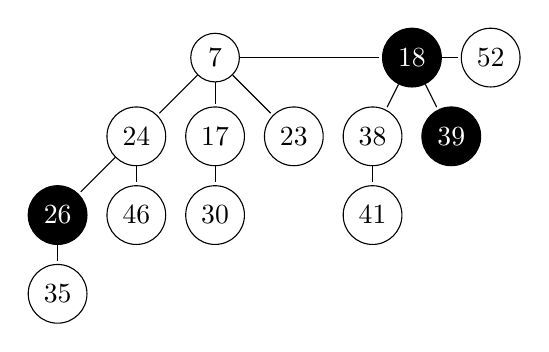
\begin{tikzpicture}[scale=0.5,shorten >=1pt]
                        % Nodes
                        \node[circle, draw] (7) at (1,0) {7};
                        \node[circle, draw] (23) at (3,-2) {23};
                        \node[circle, draw] (17) at (1,-2) {17};
                        \node[circle, draw] (30) at (1,-4) {30};
                        \node[circle, draw] (24) at (-1,-2) {24};
                        \node[circle, draw, fill=black, text=white] (26) at (-3,-4) {26};
                        \node[circle, draw] (35) at (-3,-6) {35};
                        \node[circle, draw] (46) at (-1,-4) {46};
                        \node[circle, draw, fill=black, text=white] (18) at (6,0) {18};
                        \node[circle, draw, fill=black, text=white] (39) at (7,-2) {39};
                        \node[circle, draw] (38) at (5,-2) {38};
                        \node[circle, draw] (41) at (5,-4) {41};
                        \node[circle, draw] (52) at (8,0) {52};
                        
                        % Edges
                        \draw[-] (7) -- (18);
                        \draw[-] (18) -- (52);
                        
                        \draw[-] (7) -- (23);
                        \draw[-] (7) -- (17);
                        \draw[-] (7) -- (24);
                        \draw[-] (18) -- (39);
                        \draw[-] (18) -- (38);
                        \draw[-] (38) -- (41);
                        
                        \draw[-] (17) -- (30);
                        \draw[-] (24) -- (26);
                        \draw[-] (24) -- (46);

                        \draw[-] (26) -- (35);
                    \end{tikzpicture}
                \end{figure}
            \item [Step 6.] 
                After merged, the list we recorded is [(7, 3), (18, 2)], keep moving forward and record.
                The list we recorded is [(7, 3), (18, 2), (52, 0)], the next node is (7, 3), hence the process is complete.
                \begin{figure}[!ht]
                    \centering
                    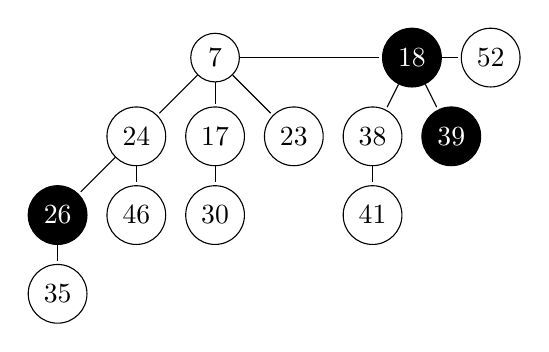
\begin{tikzpicture}[scale=0.5,shorten >=1pt]
                        % Nodes
                        \node[circle, draw] (7) at (1,0) {7};
                        \node[circle, draw] (23) at (3,-2) {23};
                        \node[circle, draw] (17) at (1,-2) {17};
                        \node[circle, draw] (30) at (1,-4) {30};
                        \node[circle, draw] (24) at (-1,-2) {24};
                        \node[circle, draw, fill=black, text=white] (26) at (-3,-4) {26};
                        \node[circle, draw] (35) at (-3,-6) {35};
                        \node[circle, draw] (46) at (-1,-4) {46};
                        \node[circle, draw, fill=black, text=white] (18) at (6,0) {18};
                        \node[circle, draw, fill=black, text=white] (39) at (7,-2) {39};
                        \node[circle, draw] (38) at (5,-2) {38};
                        \node[circle, draw] (41) at (5,-4) {41};
                        \node[circle, draw] (52) at (8,0) {52};
                        
                        % Edges
                        \draw[-] (7) -- (18);
                        \draw[-] (18) -- (52);
                        
                        \draw[-] (7) -- (23);
                        \draw[-] (7) -- (17);
                        \draw[-] (7) -- (24);
                        \draw[-] (18) -- (39);
                        \draw[-] (18) -- (38);
                        \draw[-] (38) -- (41);
                        
                        \draw[-] (17) -- (30);
                        \draw[-] (24) -- (26);
                        \draw[-] (24) -- (46);

                        \draw[-] (26) -- (35);
                    \end{tikzpicture}
                \end{figure}
        \end{enumerate}
    \item [(b)] Result:
        \begin{enumerate}
            \item [Step 1.] Decrease 35 to 2, then move 2 to root list:
                \begin{figure}[!ht]
                    \centering
                    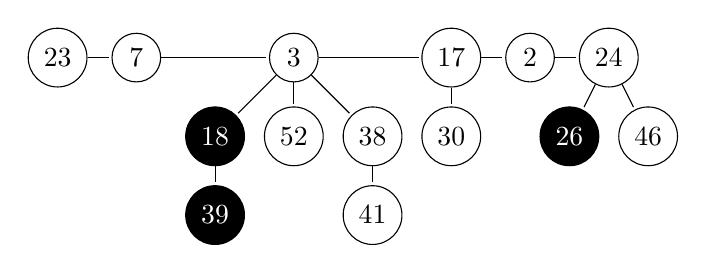
\begin{tikzpicture}[scale=0.5,shorten >=1pt]
                        % Nodes
                        \node[circle, draw] (23) at (-1,0) {23};
                        \node[circle, draw] (7) at (1,0) {7};
                        \node[circle, draw] (3) at (5,0) {3};
                        \node[circle, draw] (17) at (9,0) {17};
                        \node[circle, draw] (24) at (13,0) {24};
                        \node[circle, draw, fill=black, text=white] (18) at (3,-2) {18};
                        \node[circle, draw, fill=black, text=white] (39) at (3,-4) {39};
                        \node[circle, draw] (52) at (5,-2) {52};
                        \node[circle, draw] (38) at (7,-2) {38};
                        \node[circle, draw] (41) at (7,-4) {41};
                        \node[circle, draw] (30) at (9, -2) {30};
                        \node[circle, draw, fill=black, text=white] (26) at (12,-2) {26};
                        \node[circle, draw] (2) at (11,0) {2};
                        \node[circle, draw] (46) at (14,-2) {46};

                        % Edges
                        \draw[-] (23) -- (7);
                        \draw[-] (7) -- (3);
                        \draw[-] (3) -- (18);
                        \draw[-] (3) -- (52);
                        \draw[-] (3) -- (38);
                        \draw[-] (3) -- (17);
                        \draw[-] (17) -- (2);
                        \draw[-] (2) -- (24);
                        
                        \draw[-] (17) -- (30);
                        \draw[-] (24) -- (26);
                        \draw[-] (24) -- (46);

                        \draw[-] (18) -- (39);
                        \draw[-] (38) -- (41);
                    \end{tikzpicture}
                \end{figure}
            \item [Step 2.] 26 lost a kid, since 26 had already lost a kid, move 26 to root list and reset the lost kid number:
                \begin{figure}[!ht]
                    \centering
                    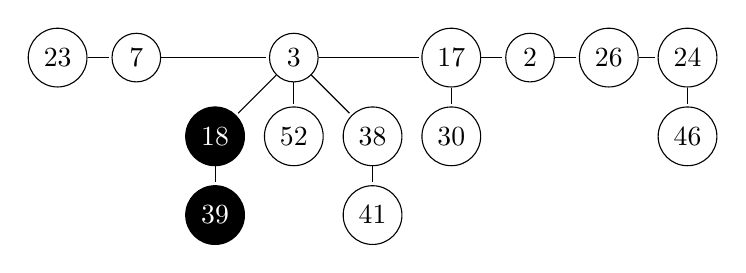
\begin{tikzpicture}[scale=0.5,shorten >=1pt]
                        % Nodes
                        \node[circle, draw] (23) at (-1,0) {23};
                        \node[circle, draw] (7) at (1,0) {7};
                        \node[circle, draw] (3) at (5,0) {3};
                        \node[circle, draw] (17) at (9,0) {17};
                        \node[circle, draw] (2) at (11,0) {2};
                        \node[circle, draw] (26) at (13,0) {26};
                        \node[circle, draw] (24) at (15,0) {24};
                        \node[circle, draw, fill=black, text=white] (18) at (3,-2) {18};
                        \node[circle, draw, fill=black, text=white] (39) at (3,-4) {39};
                        \node[circle, draw] (52) at (5,-2) {52};
                        \node[circle, draw] (38) at (7,-2) {38};
                        \node[circle, draw] (41) at (7,-4) {41};
                        \node[circle, draw] (30) at (9, -2) {30};
                        \node[circle, draw] (46) at (15,-2) {46};

                        % Edges
                        \draw[-] (23) -- (7);
                        \draw[-] (7) -- (3);
                        \draw[-] (3) -- (18);
                        \draw[-] (3) -- (52);
                        \draw[-] (3) -- (38);
                        \draw[-] (3) -- (17);
                        \draw[-] (17) -- (2);
                        \draw[-] (2) -- (26);
                        \draw[-] (26) -- (24);

                        \draw[-] (17) -- (30);
                        \draw[-] (24) -- (46);

                        \draw[-] (18) -- (39);
                        \draw[-] (38) -- (41);
                    \end{tikzpicture}
                \end{figure}
            \item [Step 3.] Change the min number to 2.
        \end{enumerate}
\end{enumerate}

\section{Modified Fibonacci Heap}

\begin{enumerate}
    \item [(a)] 
        In the modified Fibonacci heap, the node will be cascading cut only if the mark of the node reach two.
        That is, the node had lost its child two times, and now it lost its child again.
        Hence, the potential move of the modified Fibonacci heap is $\phi(H) = t(H)+2\times m_{2}(H)$, where $m_{2}(H)$ means the number of nodes which has mark = 2.
        \begin{enumerate}
            \item [i.] 
                Insertion won't change any of the $m_{2}(H)$, and $t(H)$ will increase by 1, so the cost of insertion is $\phi(H') - \phi(H) = 1$. Amortized cost: $O(1)$.
            \item [ii.]
                When we decrease key k, we will execute cut 1 time, then start cascading-cut.
                In the cascading-cut, we only execute cut when we find the node with mark = 2. Hence, cut will be executed $c \leq m_{2}(H)$ times when doing cascading-cut.
                For each cut executed, the tree number will increase by 1.
                Then the potential function $$\phi(H') \leq (t(H) + c + 1) + 2\times (m_{2}(H) - c + 1) = \phi(H) + 2 - c$$
                Hence, the amortized cost is $O(1)$.
            \item [iii.] 
                Delete-min won't change any of the $m_{2}(H)$, but the tree number will increase the children number of min node, so
                $\phi(H') - \phi(H) = D(n)$, which means the amortized cost is $O(D(n))$
            \item [iv.]
                Union only change the minimum number of the heap, so that $\phi(H') - \phi(H) = 0$. Hence, the amortized cost is $O(1)$.
        \end{enumerate}
\end{enumerate}

\section{Disjoint Set}

\begin{enumerate}
    \item [(a)]
        Result:
        \begin{figure}[!ht]
            \centering

            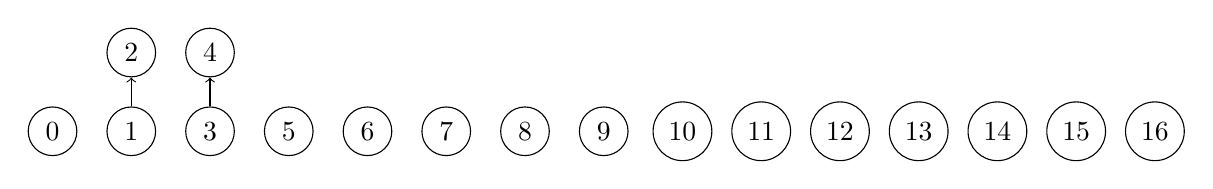
\begin{tikzpicture}
                % Nodes
                \node[circle, draw] (0) at (0,0) {0};
                \node[circle, draw] (1) at (1,0) {1};
                \node[circle, draw] (2) at (1,1) {2};
                \node[circle, draw] (3) at (2,0) {3};
                \node[circle, draw] (4) at (2,1) {4};
                \node[circle, draw] (5) at (3,0) {5};
                \node[circle, draw] (6) at (4,0) {6};
                \node[circle, draw] (7) at (5,0) {7};
                \node[circle, draw] (8) at (6,0) {8};
                \node[circle, draw] (9) at (7,0) {9};
                \node[circle, draw] (10) at (8,0) {10};
                \node[circle, draw] (11) at (9,0) {11};
                \node[circle, draw] (12) at (10,0) {12};
                \node[circle, draw] (13) at (11,0) {13};
                \node[circle, draw] (14) at (12,0) {14};
                \node[circle, draw] (15) at (13,0) {15};
                \node[circle, draw] (16) at (14,0) {16};

                % Edges
                \draw[->] (1)--(2);
                \draw[->] (3)--(4);
            \end{tikzpicture}
            \caption{union(1, 2), union(3, 4)}
        \end{figure}
        \begin{figure}[!ht]
            \centering
            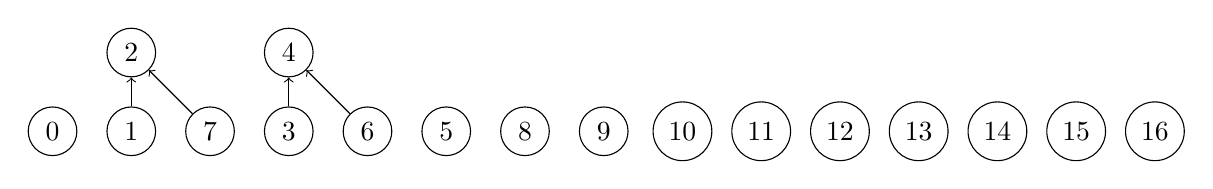
\begin{tikzpicture}
                % Nodes
                \node[circle, draw] (0) at (0,0) {0};
                \node[circle, draw] (1) at (1,0) {1};
                \node[circle, draw] (2) at (1,1) {2};
                \node[circle, draw] (3) at (3,0) {3};
                \node[circle, draw] (4) at (3,1) {4};
                \node[circle, draw] (5) at (5,0) {5};
                \node[circle, draw] (6) at (4,0) {6};
                \node[circle, draw] (7) at (2,0) {7};
                \node[circle, draw] (8) at (6,0) {8};
                \node[circle, draw] (9) at (7,0) {9};
                \node[circle, draw] (10) at (8,0) {10};
                \node[circle, draw] (11) at (9,0) {11};
                \node[circle, draw] (12) at (10,0) {12};
                \node[circle, draw] (13) at (11,0) {13};
                \node[circle, draw] (14) at (12,0) {14};
                \node[circle, draw] (15) at (13,0) {15};
                \node[circle, draw] (16) at (14,0) {16};

                % Edges
                \draw[->] (1)--(2);
                \draw[->] (3)--(4);
                \draw[->] (7)--(2);
                \draw[->] (6)--(4);
            \end{tikzpicture}
            \caption{union(1, 7), union(3, 6)}
        \end{figure}
        \begin{figure}[!ht]
            \centering
            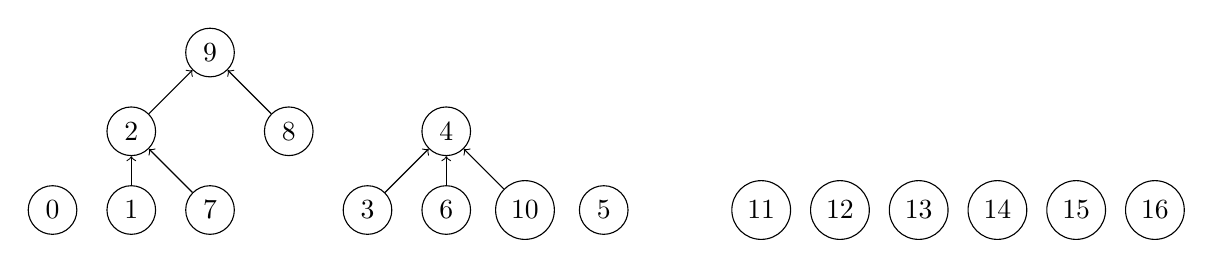
\begin{tikzpicture}
                % Nodes
                \node[circle, draw] (0) at (0,0) {0};
                \node[circle, draw] (1) at (1,0) {1};
                \node[circle, draw] (2) at (1,1) {2};
                \node[circle, draw] (3) at (4,0) {3};
                \node[circle, draw] (4) at (5,1) {4};
                \node[circle, draw] (5) at (7,0) {5};
                \node[circle, draw] (6) at (5,0) {6};
                \node[circle, draw] (7) at (2,0) {7};
                \node[circle, draw] (8) at (3,1) {8};
                \node[circle, draw] (9) at (2,2) {9};
                \node[circle, draw] (10) at (6,0) {10};
                \node[circle, draw] (11) at (9,0) {11};
                \node[circle, draw] (12) at (10,0) {12};
                \node[circle, draw] (13) at (11,0) {13};
                \node[circle, draw] (14) at (12,0) {14};
                \node[circle, draw] (15) at (13,0) {15};
                \node[circle, draw] (16) at (14,0) {16};

                % Edges
                \draw[->] (1)--(2);
                \draw[->] (3)--(4);
                \draw[->] (7)--(2);
                \draw[->] (6)--(4);
                \draw[->] (8)--(9);
                \draw[->] (2)--(9);
                \draw[->] (10)--(4);
            \end{tikzpicture}
            \caption{union(8, 9) then union(1, 8), union(3, 10)}
        \end{figure}
        \begin{figure}[!ht]
            \centering
            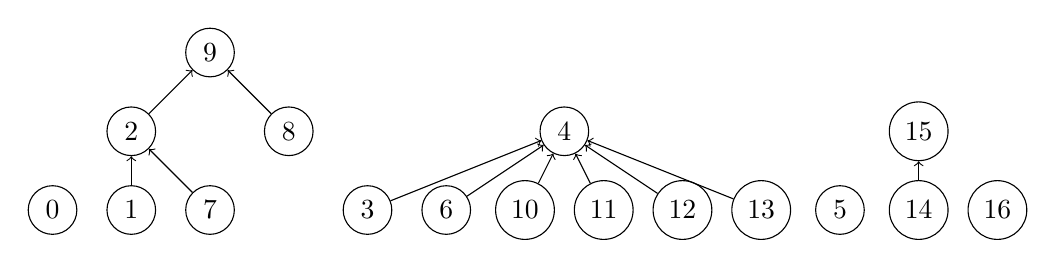
\begin{tikzpicture}
                % Nodes
                \node[circle, draw] (0) at (0,0) {0};
                \node[circle, draw] (1) at (1,0) {1};
                \node[circle, draw] (2) at (1,1) {2};
                \node[circle, draw] (3) at (4,0) {3};
                \node[circle, draw] (4) at (6.5,1) {4};
                \node[circle, draw] (5) at (10,0) {5};
                \node[circle, draw] (6) at (5,0) {6};
                \node[circle, draw] (7) at (2,0) {7};
                \node[circle, draw] (8) at (3,1) {8};
                \node[circle, draw] (9) at (2,2) {9};
                \node[circle, draw] (10) at (6,0) {10};
                \node[circle, draw] (11) at (7,0) {11};
                \node[circle, draw] (12) at (8,0) {12};
                \node[circle, draw] (13) at (9,0) {13};
                \node[circle, draw] (14) at (11,0) {14};
                \node[circle, draw] (15) at (11,1) {15};
                \node[circle, draw] (16) at (12,0) {16};

                % Edges
                \draw[->] (1)--(2);
                \draw[->] (3)--(4);
                \draw[->] (7)--(2);
                \draw[->] (6)--(4);
                \draw[->] (8)--(9);
                \draw[->] (2)--(9);
                \draw[->] (10)--(4);
                \draw[->] (11)--(4);
                \draw[->] (12)--(4);
                \draw[->] (13)--(4);
                \draw[->] (14)--(15);
            \end{tikzpicture}
            \caption{union(3, 11), union(3, 12), union(3, 13), union(14, 15)}
        \end{figure}
        \begin{figure}[!ht]
            \centering
            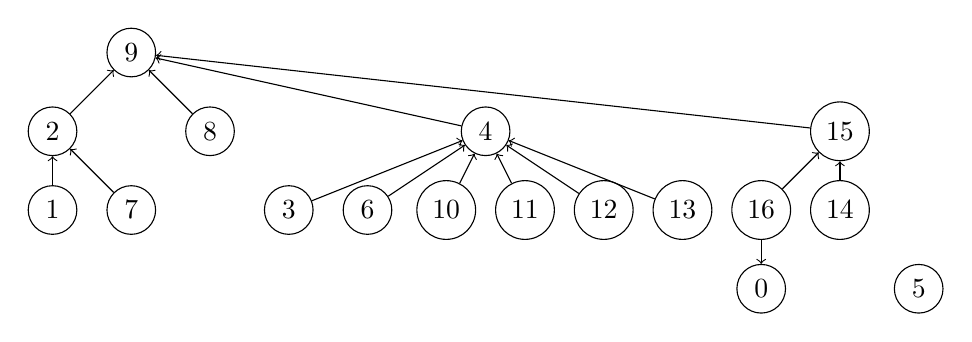
\begin{tikzpicture}
                % Nodes
                \node[circle, draw] (0) at (10,0) {0};
                \node[circle, draw] (1) at (1,1) {1};
                \node[circle, draw] (2) at (1,2) {2};
                \node[circle, draw] (3) at (4,1) {3};
                \node[circle, draw] (4) at (6.5,2) {4};
                \node[circle, draw] (5) at (12,0) {5};
                \node[circle, draw] (6) at (5,1) {6};
                \node[circle, draw] (7) at (2,1) {7};
                \node[circle, draw] (8) at (3,2) {8};
                \node[circle, draw] (9) at (2,3) {9};
                \node[circle, draw] (10) at (6,1) {10};
                \node[circle, draw] (11) at (7,1) {11};
                \node[circle, draw] (12) at (8,1) {12};
                \node[circle, draw] (13) at (9,1) {13};
                \node[circle, draw] (14) at (11,1) {14};
                \node[circle, draw] (15) at (11,2) {15};
                \node[circle, draw] (16) at (10,1) {16};

                % Edges
                \draw[->] (1)--(2);
                \draw[->] (3)--(4);
                \draw[->] (7)--(2);
                \draw[->] (6)--(4);
                \draw[->] (8)--(9);
                \draw[->] (2)--(9);
                \draw[->] (10)--(4);
                \draw[->] (11)--(4);
                \draw[->] (12)--(4);
                \draw[->] (13)--(4);
                \draw[->] (14)--(15);
                \draw[->] (16)--(0);
                \draw[->] (16)--(15);
                \draw[->] (4)--(9);
                \draw[->] (15)--(9);
            \end{tikzpicture}
            \caption{union(16, 0), union(14, 16), union(1, 3), union(1, 14)}
        \end{figure}
    \newpage
    \item [(b)]
        Result:
        \begin{figure}[!ht]
            \centering

            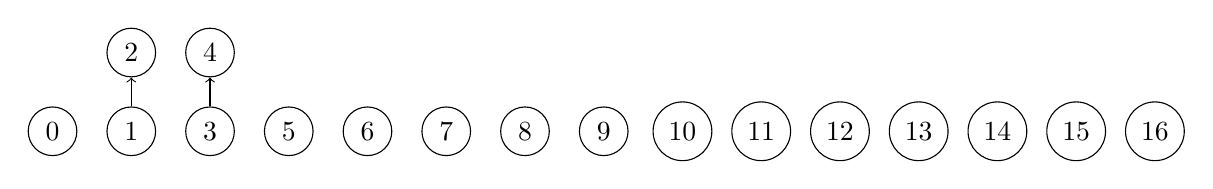
\begin{tikzpicture}
                % Nodes
                \node[circle, draw] (0) at (0,0) {0};
                \node[circle, draw] (1) at (1,0) {1};
                \node[circle, draw] (2) at (1,1) {2};
                \node[circle, draw] (3) at (2,0) {3};
                \node[circle, draw] (4) at (2,1) {4};
                \node[circle, draw] (5) at (3,0) {5};
                \node[circle, draw] (6) at (4,0) {6};
                \node[circle, draw] (7) at (5,0) {7};
                \node[circle, draw] (8) at (6,0) {8};
                \node[circle, draw] (9) at (7,0) {9};
                \node[circle, draw] (10) at (8,0) {10};
                \node[circle, draw] (11) at (9,0) {11};
                \node[circle, draw] (12) at (10,0) {12};
                \node[circle, draw] (13) at (11,0) {13};
                \node[circle, draw] (14) at (12,0) {14};
                \node[circle, draw] (15) at (13,0) {15};
                \node[circle, draw] (16) at (14,0) {16};

                % Edges
                \draw[->] (1)--(2);
                \draw[->] (3)--(4);
            \end{tikzpicture}
            \caption{union(1, 2), union(3, 4)}
        \end{figure}
        \begin{figure}[!ht]
            \centering
            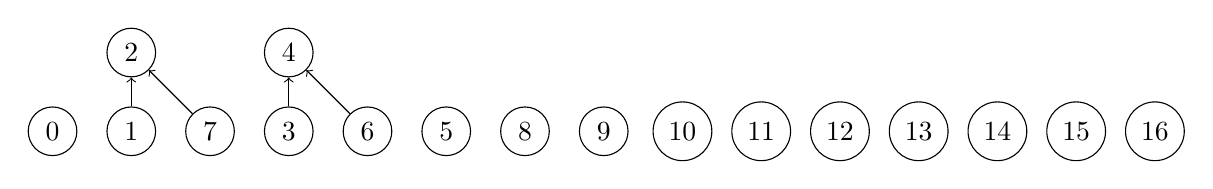
\begin{tikzpicture}
                % Nodes
                \node[circle, draw] (0) at (0,0) {0};
                \node[circle, draw] (1) at (1,0) {1};
                \node[circle, draw] (2) at (1,1) {2};
                \node[circle, draw] (3) at (3,0) {3};
                \node[circle, draw] (4) at (3,1) {4};
                \node[circle, draw] (5) at (5,0) {5};
                \node[circle, draw] (6) at (4,0) {6};
                \node[circle, draw] (7) at (2,0) {7};
                \node[circle, draw] (8) at (6,0) {8};
                \node[circle, draw] (9) at (7,0) {9};
                \node[circle, draw] (10) at (8,0) {10};
                \node[circle, draw] (11) at (9,0) {11};
                \node[circle, draw] (12) at (10,0) {12};
                \node[circle, draw] (13) at (11,0) {13};
                \node[circle, draw] (14) at (12,0) {14};
                \node[circle, draw] (15) at (13,0) {15};
                \node[circle, draw] (16) at (14,0) {16};

                % Edges
                \draw[->] (1)--(2);
                \draw[->] (3)--(4);
                \draw[->] (7)--(2);
                \draw[->] (6)--(4);
            \end{tikzpicture}
            \caption{union(1, 7), union(3, 6)}
        \end{figure}
        \begin{figure}[!ht]
            \centering
            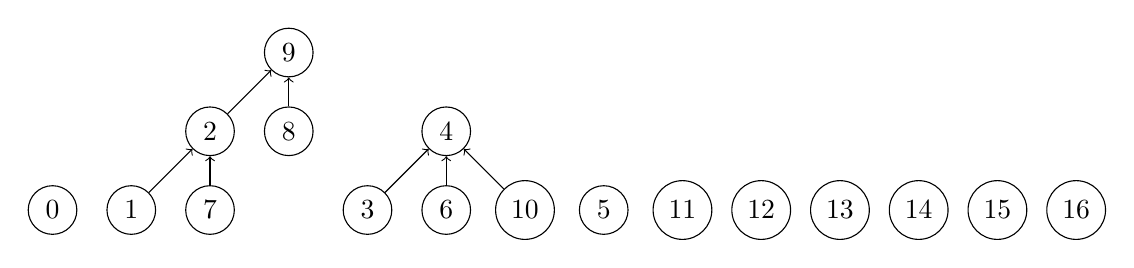
\begin{tikzpicture}
                % Nodes
                \node[circle, draw] (0) at (-1,0) {0};
                \node[circle, draw] (1) at (0,0) {1};
                \node[circle, draw] (2) at (1,1) {2};
                \node[circle, draw] (3) at (3,0) {3};
                \node[circle, draw] (4) at (4,1) {4};
                \node[circle, draw] (5) at (6,0) {5};
                \node[circle, draw] (6) at (4,0) {6};
                \node[circle, draw] (7) at (1,0) {7};
                \node[circle, draw] (8) at (2,1) {8};
                \node[circle, draw] (9) at (2,2) {9};
                \node[circle, draw] (10) at (5,0) {10};
                \node[circle, draw] (11) at (7,0) {11};
                \node[circle, draw] (12) at (8,0) {12};
                \node[circle, draw] (13) at (9,0) {13};
                \node[circle, draw] (14) at (10,0) {14};
                \node[circle, draw] (15) at (11,0) {15};
                \node[circle, draw] (16) at (12,0) {16};

                % Edges
                \draw[->] (1)--(2);
                \draw[->] (3)--(4);
                \draw[->] (7)--(2);
                \draw[->] (6)--(4);
                \draw[->] (8)--(9);
                \draw[->] (2)--(9);
                \draw[->] (10)--(4);
            \end{tikzpicture}
            \caption{union(8, 9) then union(1, 8), union(3, 10)}
        \end{figure}
        \begin{figure}[!ht]
            \centering
            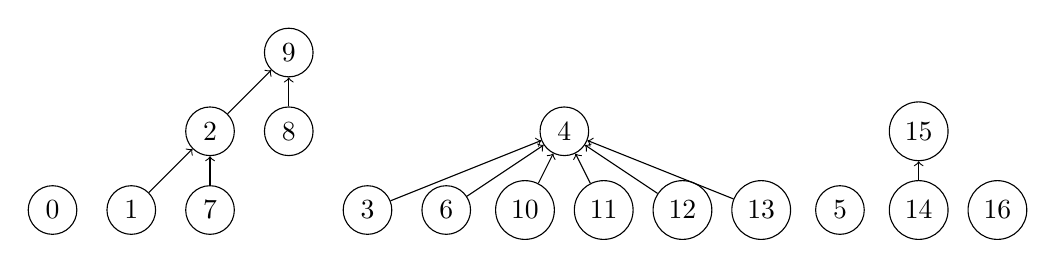
\begin{tikzpicture}
                % Nodes
                \node[circle, draw] (0) at (-1,0) {0};
                \node[circle, draw] (1) at (0,0) {1};
                \node[circle, draw] (2) at (1,1) {2};
                \node[circle, draw] (3) at (3,0) {3};
                \node[circle, draw] (4) at (5.5,1) {4};
                \node[circle, draw] (5) at (9,0) {5};
                \node[circle, draw] (6) at (4,0) {6};
                \node[circle, draw] (7) at (1,0) {7};
                \node[circle, draw] (8) at (2,1) {8};
                \node[circle, draw] (9) at (2,2) {9};
                \node[circle, draw] (10) at (5,0) {10};
                \node[circle, draw] (11) at (6,0) {11};
                \node[circle, draw] (12) at (7,0) {12};
                \node[circle, draw] (13) at (8,0) {13};
                \node[circle, draw] (14) at (10,0) {14};
                \node[circle, draw] (15) at (10,1) {15};
                \node[circle, draw] (16) at (11,0) {16};

                % Edges
                \draw[->] (1)--(2);
                \draw[->] (3)--(4);
                \draw[->] (7)--(2);
                \draw[->] (6)--(4);
                \draw[->] (8)--(9);
                \draw[->] (2)--(9);
                \draw[->] (10)--(4);
                \draw[->] (11)--(4);
                \draw[->] (12)--(4);
                \draw[->] (13)--(4);
                \draw[->] (14)--(15);
            \end{tikzpicture}
            \caption{union(3, 11), union(3, 12), union(3, 13), union(14, 15)}
        \end{figure}
        \begin{figure}[!ht]
            \centering
            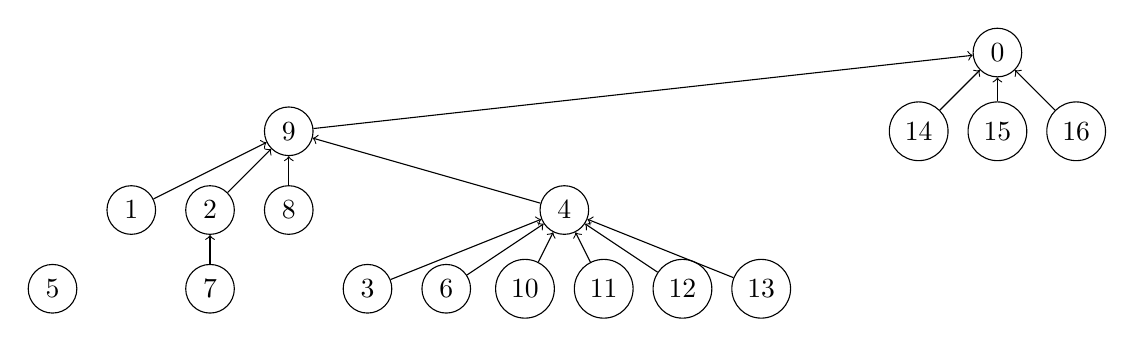
\begin{tikzpicture}
                % Nodes
                \node[circle, draw] (0) at (11,3) {0};
                \node[circle, draw] (1) at (0,1) {1};
                \node[circle, draw] (2) at (1,1) {2};
                \node[circle, draw] (3) at (3,0) {3};
                \node[circle, draw] (4) at (5.5,1) {4};
                \node[circle, draw] (5) at (-1,0) {5};
                \node[circle, draw] (6) at (4,0) {6};
                \node[circle, draw] (7) at (1,0) {7};
                \node[circle, draw] (8) at (2,1) {8};
                \node[circle, draw] (9) at (2,2) {9};
                \node[circle, draw] (10) at (5,0) {10};
                \node[circle, draw] (11) at (6,0) {11};
                \node[circle, draw] (12) at (7,0) {12};
                \node[circle, draw] (13) at (8,0) {13};
                \node[circle, draw] (14) at (10,2) {14};
                \node[circle, draw] (15) at (11,2) {15};
                \node[circle, draw] (16) at (12,2) {16};

                % Edges
                \draw[->] (1)--(9);
                \draw[->] (3)--(4);
                \draw[->] (7)--(2);
                \draw[->] (6)--(4);
                \draw[->] (8)--(9);
                \draw[->] (2)--(9);
                \draw[->] (10)--(4);
                \draw[->] (11)--(4);
                \draw[->] (12)--(4);
                \draw[->] (13)--(4);
                \draw[->] (14)--(0);
                \draw[->] (16)--(0);
                \draw[->] (15)--(0);
                \draw[->] (4)--(9);
                \draw[->] (9)--(0);
            \end{tikzpicture}
            \caption{union(16, 0), union(14, 16), union(1, 3), union(1, 14)}
        \end{figure}
\end{enumerate}

\newpage

\section{Disjoint Set Algorithm}

Add another attribute link, and change the functions MAKE-SET, LINK, PRINT-SET. Then we can reach the goal we want.

\begin{algorithm}
    \caption{Print-Set(x)}
    \KwIn{x}
    \KwOut{print the set of x}
    \SetKwFunction{FMain}{MAKE-SET}
    \SetKwProg{Fn}{Function}{:}{}
    \Fn{\FMain{$x$}}{
        $ x.parent  \longleftarrow x $;\\
        $ x.rank  \longleftarrow 0 $;\\
        $ x.link  \longleftarrow x $;\\
    }
    \textbf{End Function}\\
    \SetKwFunction{FMain}{LINK}
    \SetKwProg{Fn}{Function}{:}{}
    \Fn{\FMain{$x, y$}}{
        $ temp = y.link $;\\
        $ y.link = x.link $;\\
        $ x.link = temp $;\\
        \uIf{$x.rank > y.rank$}
        {
            $ y.parent  \longleftarrow x $;\\
        }
        \uElse
        {
            $ x.parent  \longleftarrow y $;\\
        }
    }
    \textbf{End Function}\\
    \SetKwFunction{FMain}{PRINT-SET}
    \SetKwProg{Fn}{Function}{:}{}
    \Fn{\FMain{$x$}}{
        $ root = x $;\\
        \While{$ x.link \neq root$}
        {
            print($x$);\\
            $x \longleftarrow x.link$;
        }
        print($x$);
    }
\end{algorithm}

\end{document}
